% \VignetteIndexEntry{The otsad Package: Online Time-Series Anomaly Detectors}
% \VignetteDepends{otsad}
% \VignetteKeywords{otsad}
% \VignetteKeywords{anomaly time serie}
% \VignettePackage{otsad}
%\VignetteCompiler{knitr}
%\VignetteEngine{knitr::knitr}

\documentclass[a4paper]{article}\usepackage[]{graphicx}\usepackage[]{color}
% maxwidth is the original width if it is less than linewidth
% otherwise use linewidth (to make sure the graphics do not exceed the margin)
\makeatletter
\def\maxwidth{ %
  \ifdim\Gin@nat@width>\linewidth
    \linewidth
  \else
    \Gin@nat@width
  \fi
}
\makeatother

\definecolor{fgcolor}{rgb}{0.345, 0.345, 0.345}
\newcommand{\hlnum}[1]{\textcolor[rgb]{0.686,0.059,0.569}{#1}}%
\newcommand{\hlstr}[1]{\textcolor[rgb]{0.192,0.494,0.8}{#1}}%
\newcommand{\hlcom}[1]{\textcolor[rgb]{0.678,0.584,0.686}{\textit{#1}}}%
\newcommand{\hlopt}[1]{\textcolor[rgb]{0,0,0}{#1}}%
\newcommand{\hlstd}[1]{\textcolor[rgb]{0.345,0.345,0.345}{#1}}%
\newcommand{\hlkwa}[1]{\textcolor[rgb]{0.161,0.373,0.58}{\textbf{#1}}}%
\newcommand{\hlkwb}[1]{\textcolor[rgb]{0.69,0.353,0.396}{#1}}%
\newcommand{\hlkwc}[1]{\textcolor[rgb]{0.333,0.667,0.333}{#1}}%
\newcommand{\hlkwd}[1]{\textcolor[rgb]{0.737,0.353,0.396}{\textbf{#1}}}%
\let\hlipl\hlkwb

\usepackage{framed}
\makeatletter
\newenvironment{kframe}{%
 \def\at@end@of@kframe{}%
 \ifinner\ifhmode%
  \def\at@end@of@kframe{\end{minipage}}%
  \begin{minipage}{\columnwidth}%
 \fi\fi%
 \def\FrameCommand##1{\hskip\@totalleftmargin \hskip-\fboxsep
 \colorbox{shadecolor}{##1}\hskip-\fboxsep
     % There is no \\@totalrightmargin, so:
     \hskip-\linewidth \hskip-\@totalleftmargin \hskip\columnwidth}%
 \MakeFramed {\advance\hsize-\width
   \@totalleftmargin\z@ \linewidth\hsize
   \@setminipage}}%
 {\par\unskip\endMakeFramed%
 \at@end@of@kframe}
\makeatother

\definecolor{shadecolor}{rgb}{.97, .97, .97}
\definecolor{messagecolor}{rgb}{0, 0, 0}
\definecolor{warningcolor}{rgb}{1, 0, 1}
\definecolor{errorcolor}{rgb}{1, 0, 0}
\newenvironment{knitrout}{}{} % an empty environment to be redefined in TeX

\usepackage{alltt}
%\documentclass[article, 5p, 10pt]{elsarticle}
\usepackage[utf8]{inputenc}
%\usepackage[T1]{fontenc}
\usepackage{amsmath,amssymb,array}
\usepackage{booktabs}

% Size of the layout
\usepackage[a4paper, total={160mm, 247mm}]{geometry}

%% load any required packages here

\usepackage{color}
\usepackage{stmaryrd}
\usepackage{url}
\usepackage[numbers,sectionbib]{natbib}

\usepackage{authblk}
\usepackage{epstopdf}

\usepackage{booktabs}
\usepackage{multirow}
\IfFileExists{upquote.sty}{\usepackage{upquote}}{}
\begin{document}

\providecommand{\pkg}[1]{\textbf{#1}}
\providecommand{\CRANpkg}[1]{\textbf{#1}}
\providecommand{\code}[1]{\texttt{#1}}
\providecommand{\file}[1]{\texttt{'#1'}}

\title{The \pkg{otsad} Package:\\ Online Time-Series Anomaly Detectors}

%\author{Alaiñe Iturria}

\author[1,2]{Alaiñe Iturria}
\author[2]{Jacinto Carrasco}
\author[2]{Francisco Herrera}
\author[1]{Santi Charramendieta}
\author[1]{Karmele Intxausti}

\affil[1]{IK4-Ikerlan, Big Data Architectures Team, Paseo J.Mª Arizmediarrieta, 2, 20500 Arrasate-Mondragon. Spain}
\affil[2]{Department of Computer Science and Artificial Intelligence, University of Granada, Granada, 18071, Spain}


\date{}

\maketitle

\definecolor{highlight}{rgb}{0,0,0}


\abstract{
Anomaly detection gives valuable information that can be used to solve malfunctions and prevent future problems. Although this field has been widely studied, due to the continuous evolution of technology, new challenges arise that require further improvement and evolution of anomaly detection techniques. In this paper, we present the \pkg{ostad} package that implements seven of the most recent detection algorithms capable of dealing with various challenges, such as online and non-stationary univariate time-series anomaly detection.
}

\section{Introduction}

Anomaly detection consists of the identification of patterns in the data that differ from expected behavior and is a relevant task in many domains such as fault detection in the manufacturing industry, intrusion detection in cybersecurity and fraud detection in banks. Anomaly detection is an extensive field that has been studied for years. Chandola et al.  \cite{Chandola}, Hodge et al. \cite{Hodge} and Zhang et al. \cite{Zhang} provide a comprehensive overview of anomaly detection techniques.

Due to the evolution of new technologies, the amount of data is increasing and is collected faster. For this reason, detection techniques must face new challenges such as an increase in the amount of data and online processing capacity. Unlike classic techniques, online time-series anomaly detection techniques do not have the complete data set to work with, and time must be considered. Another major challenge with the introduction of online time-series processing is that time-series can be stationary and non-stationary.

In recent years, most of the work has focused on the evolution of evolving prediction models and sliding window-based techniques \cite{a3e0f1cf080343d98cae7430cd6e43c4}. Evolving techniques are models in which parameters or components are modified as new data arrives to capture normal data trends in a better way. On the other hand, techniques based on sliding windows are commonly used to improve distance-based techniques. The distance calculation is an expensive method and proportional to the number of observations to be considered. The use of sliding windows allows reducing the set of observations to be considered but also maintaining the most recent subset of data.

Some works \cite{aggarwal_outlier}\cite{Blazquez-Garcia2020}, suggest that prediction-based algorithms are suitable to adapt to online time-series anomaly detection since only the past data is required during the training phase. Moreover, real-time time series prediction is an independent domain whose research is currently more advanced than TSOD. However, the continuous change of the training data set, the non-stationarity of the data, and the lack of the entire data set make it challenging to adapt the online prediction algorithms into an outlier detection. Hence, little research has been done in this domain  \cite{Ahmad2017}\cite{Xu2017}.

When adapting prediction algorithms to anomaly detection, two challenges must be addressed. The first challenge is the online anomaly scoring based on the prediction error. The techniques used in offline processing algorithms rely on the entire data set to compute the score from the prediction errors, and very few are proposed for online processing \cite{Ahmad2017}\cite{Buda2018}. The second challenge is the streaming input data normalization. Standardization or normalization of the data becomes an essential requirement for some online prediction algorithms, such as those based on neural networks \cite{Liang2006}\cite{Park2017}. However, none of them address online normalization, and they assume that data is already normalized. This is not a realistic assumption, as, in a real scenario where data arrives in real-time, the entry data set is not available. Hence, the statistics needed for normalization, e.g., minimum, maximum, mean, or deviation, may change over time, making these algorithms not suitable for real online learning tasks.

Although anomaly detection is a highly studied field, there is little theory and open-source software able to address these new challenges. For python, we have found a few algorithms in GitHub of \emph{Numenta Anomaly Benchmark (NAB)} \cite{7424283} including \textbf{Numenta HTM}, \textbf{CAD-OSE}, \textbf{KNN-CAD}, and others. For R, there are few CRAN packages. The first and most popular is the \CRANpkg{tsoutliers} package. There is also the \CRANpkg{qicharts} package that implements basic control chart algorithms. One of the main disadvantages of these packages is that the implemented algorithms are not suitable to work online. In addition to the above, there are few other packages available for online time-series anomaly detection: \CRANpkg{SmartSifter} and \CRANpkg{EnergyOnlineCPM}.

This paper presents a novel R package that includes up-to-date and powerful anomaly detection algorithms for univariate time series. Named as \pkg{ostad}, it aims to provide algorithms that cover different current needs such as online processing and the ability to work in stationary and non-stationary environments. This package intends to address both evolving and sliding window-based techniques that are gaining strength, including algorithms of both types. Moreover, to help increase the number of proposed algorithms and further progress in this field, this work aims to provide a novel framework that allows an easy adaptation of any online prediction algorithm into an online TSOD. The framework covers these two crucial aspects: streaming normalization and outlier scoring. It contains two main components. The first component is oriented to online data normalization or standardization, while the second focuses on online anomaly scoring based on prediction errors. Both components implement several online normalization and outlier scoring methods already available in state-of-the-art and new proposals.

The rest of the paper is organized as follows. The following section introduces the content of the \pkg{otsad} package, while section \ref{sec:examplesec} describes in detail how to use implemented detectors and reduce false positives. Finally, we conclude the paper with some conclusions and future lines for continuing the work, section \ref{sec:summary}.

\section{The \pkg{otsad} package}\label{sec:package}

This section introduces the first R package that develops a set of up-to-date and effective online anomaly detectors for univariate time series. The \pkg{otsad} package implements eight anomaly detection algorithms along with other functionalities and contents that can be interesting to adapt online time-series forecasting algorithms and perform the best results.

For an easier understanding of this section, we divided it into five subsections. In the first subsection, we described each implemented algorithms. A novel detector evaluation technique is presented in section \ref{sec:measure}. Then, we introduce included datasets and the function to visualize the results in section \ref{sec:display}. After that, section \ref{sec:fp} describes a simple but effective technique for reducing false positives. Finally, in section \ref{sec:framework} a framework for easily adapting any online prediction model to outlier detection is introduced.

\subsection{Anomaly detection algorithms} \label{sec:detectors}

This package implements and documents the set of detectors listed below. The first three algorithms belong to evolving-based techniques, and the last four belong to window-based ones. From a stationary environment perspective, the first two algorithms can be used with stationary data, while the other five are suitable for non-stationary data. Table \ref{tab:features} shows the most important characteristics of each algorithm.

\begin{itemize}

\item \emph{PEWMA} or \emph{Probabilistic reasoning for streaming anomaly detection} \cite{pewma}. This algorithm is a probabilistic method of EWMA which dynamically adjusts the parameters based on the probability of the given observation. This method produces dynamic, data-driven anomaly thresholds robust to abrupt transient changes yet quickly adjust to long-term distributional shifts.

\item \emph{SD-EWMA} or \emph{Shift-Detection based on EWMA} \cite{Raza}. This algorithm is a novel method for covariate shift-detection tests using univariate time-series. It uses an exponentially weighted moving average (EWMA) model based control chart to detect the covariate shift-point in stationary time-series. SD-EWMA algorithm works in an online mode.

\item \emph{TSSD-EWMA} or \emph{Two-Stage Shift-Detection based on EWMA} \cite{Raza}. This algorithm is a novel method for covariate shift-detection tests based on a two-stage structure for univariate time-series. It uses an exponentially weighted moving average (EWMA) model-based control chart to detect the covariate shift-point in non-stationary time-series. The algorithm works in two phases and processes the stream in an online mode. In the first phase, it applies SD-EWMA. The second phase checks the anomalies' authenticity using the Kolmogorov-Simirnov test to reduce false alarms.

\item \emph{KNN-CAD} or \emph{Conformal k-NN Anomaly Detector} \cite{2016arXiv160804585B}. This algorithm is a model-free anomaly detection method for univariate time-series. It adapts itself to non-stationarity in the data stream and provides probabilistic abnormality scores based on the conformal prediction paradigm.

\item \emph{KNN-LDCD} or \emph{KNN - Lazy Drifting Conformal Detector} \cite{2017arXiv170603412I}. This algorithm is a variant of the KNN-CAD algorithm. The differences between both rely on the dissimilarity measure calculation and conformity measure calculation methods. The KNN-CAD and KNN-LDCD algorithms use both distance-based and statistical techniques to determine the degree of anomaly.

\item \emph{CAD-OSE} or \emph{Contextual Anomaly Detector} \cite{2018-Smirnov-ContextualAnomalyDetector}. This algorithm discretizes the search space and creates contexts with aggrupations of observations. When a new instance arrives, the algorithm searches in the previous storage contexts if the instance has been seen and creates a new context if it has not. The creation of new and storage contexts determines if the instance is an anomaly.

\item \emph{EORELM-AD} or \emph{Ensemble based Online Recurrent Extreme Learning Machine Anomaly Detector}. This is an ensemble of the OR-ELM prediction algorithm. The OR-ELM \cite{Park2017} is an improvement of the popular Online Sequential Extreme Learning Machine (OS-ELM)[6] that trains single-hidden layer feedforward recurrent neural networks in an online manner. EORELM-AD combines the resultant predictions of different instances of the OR-ELM algorithm for posterior anomaly scoring and detection based on prediction errors.

\end{itemize}

% Please add the following required packages to your document preamble:
% \usepackage{booktabs}
% \usepackage{multirow}
\begin{table}[]
\centering
\begin{tabular}{@{}ccc@{}}
\toprule
\multirow{2}{*}{\begin{tabular}[c]{@{}c@{}}Online anomaly\\  detectors\end{tabular}} & \multicolumn{2}{c}{Features}  \\ \cmidrule(l){2-3}
                                                                                     & Stationarity   & Technique    \\ \midrule
PEWMA                                                                                & Stationary     & Evolving   \\
SD-EWMA                                                                              & Stationary     & Evolving   \\
TSSD-EWMA                                                                            & Non-stationary & Evolving   \\
KNN-CAD                                                                              & Non-stationary & Window-based \\
KNN-LDCD                                                                             & Non-stationary & Window-based  \\
CAD-OSE                                                                              & Non-stationary & Window-based \\
EORELM-AD                                                                            & Non-stationary & Window-based \\
\bottomrule
\end{tabular}
\caption{Features of the algorithms}
\label{tab:features}

\end{table}

Each of these algorithms was implemented to work in two different scenarios. On the one hand, classical processing is used when the complete data set (train and test) is available. On the other hand, incremental (or online) processing is used when the entire dataset is unavailable. This approach allows calculating the abnormality of new observation(s) with the parameters updated in the last run performed.

\subsection{Detector measurement technique} \label{sec:measure}

The \pkg{otsad} package implements the method used in NAB \cite{7424283} to measure the detector. This method considers the time elapsed until the anomalies are detected.

This metric uses time windows to determine the label of the detected anomaly, i.e., True Positive (TP), False Positive (FP), True Negative (TN), and False Negative (FN). The label is determined by centering a window on the real anomaly. The detected anomaly is labeled as TP when it falls inside the window and as FP when it is outside. An FN label is considered when there are no detected anomalies inside the window. TN labels are not considered. The window size is calculated as the division between 10\% of the number of observations and real anomalies in the time series. The package includes three functions to perform these tasks. On the one hand, \textbf{GetWindowLength} and \textbf{GetWindowsLimits} get the size and the start and end limits of the window after being focused on the real anomalies. On the other hand, \textbf{GetLabels} gets the TP, FP, TN, and FN labels.

This measurement technique also allows setting a weight for each of these labels. These weights make it possible to penalize FN and FP and reward early detections. In this way, the FN and FP will get a negative score, and the early detections will get a higher score than the late ones, as is shown in Figure \ref{fig:ScoringEx}. NAB \cite{7424283} proposes to use the weights given in Table \ref{tab:profile}. There are three different profiles \emph{Standard}, \emph{Reward low FP rate} and \emph{Reward low FN rate}. Each one of these profiles penalizes more or less the score of FP and FN. Finally, the total score is calculated as the sum of the scores assigned to each detected anomaly and the cumulative scores of missed anomalies. This score is then scaled using the Max-Min normalization as in Equation \ref{eq:eq1}. The maximum value used is the score of a perfect detector, i.e., detects all anomalies with maximum score. The minimum value is the score of a null detector, i.e., one that does not detect any anomaly (and no FP). The final score is in the interval $(-\infty, 100]$.

For these latest objectives, we have extended the package capabilities in three more functions. First one is \textbf{GetDetectorScore}, that calculates the detector score without normalizing. The second one is \textbf{GetNullAndPerfectScores} function to obtain the scores of the perfect and null detectors for the dataset. The third one is the \textbf{NormalizeScore} function which allows normalizing detector scores.

\begin{equation}\label{eq:eq1}
Score_{final} = 100 \frac{Score_{detector} - Score_{null}}{Score_{perfect} - Score_{null}}
\end{equation}

This package incorporates an additional function to allow the user to reproduce the results of the benchmarking. Named as \textbf{GetNumTrainingValues}, this function enables obtaining the number of instances used as a training set in NAB \cite{7424283}. The number of training set values is calculated as 15\% of 5000. and for smaller datasets of 5000 instances as 15\% of the dataset instances.

% \usepackage[table,xcdraw]{xcolor}

\begin{table}[]
\caption{Label weights per profile}
\label{tab:profile}
\centering
\begin{tabular}{cccc}
\hline
\multirow{2}{*}{Label} & \multicolumn{3}{c}{Profile} \\ \cline{2-4}
 & \textbf{Standard} & \textbf{Reward low FP rate} & \textbf{Reward low FN} \\ \hline
\textbf{ATP} & 1.0 & 1.0 & 1.0 \\ \hline
\textbf{AFP} & -0.11 & -0.22 & -0.11 \\ \hline
\textbf{ATN} & 1.0 & 1.0 & 1.0 \\ \hline
\textbf{AFN} & -1.0 & -1.0 & -2.0 \\ \hline
\end{tabular}
\end{table}

\begin{figure}[htbp]
\centering
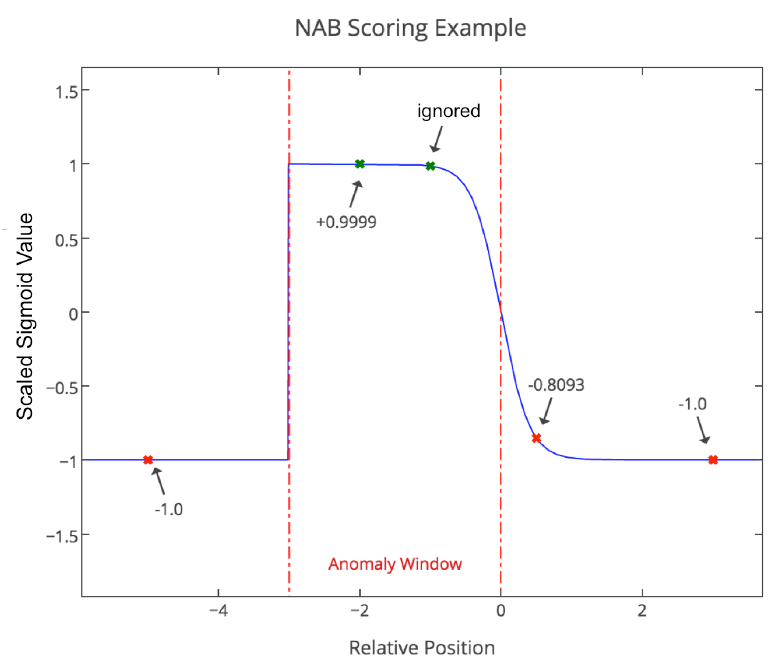
\includegraphics[width=0.7\linewidth]{ScoreExample.PNG}
\caption{Scoring example for a sample anomaly window, where the values represent the scaled sigmoid function. The first point is an FP preceding the anomaly window (red dashed lines) and contributes -1.0 to the score. Within the window, we see two detections, and only count the earliest TP for the score. There are two FPs after the window. The first is less detrimental because it is close to the window, and the second yields -1.0 because it's too far after the window to be associated with the true anomaly. TNs make no score contributions. The scaled sigmoid values are multiplied by the relevant application profile weight, the NAB score for this example would calculate as \( -1.0 A_{FP} + 0.9999 A_{TP} - 0.8093 A_{FP} - 1.0 A_{FP}\). With the standard application profile, this would result in a total score of 0.6909 \cite{7424283}}.
\label{fig:ScoringEx}
\end{figure}

\subsection{Data sets and function for displaying the results} \label{sec:display}

\pkg{Otsad} includes 51 of the 58 labeled one-dimensional time-series from different fields available in the NAB \cite{7424283} repository. Each of the datasets included in \pkg{otsad} is composed of three columns: the \emph{timestamp} column, the \emph{value} column and a third column called \emph{is.real.anomaly} containing the labeled truth anomalies.

Our package also includes a function called \textbf{PlotDetections} to display the detections results on a chart. This function, by default, returns an interactive graph, but it also has a choice to get a ggplot object, and it could be edited.

\subsection{False positive reduction technique} \label{sec:fp}

Some algorithms already included techniques to reduce false positives. These can be only applied to the above algorithms. For this reason, we introduce and implement our own algorithm, \emph{ReduceAnomalies}, to reduce false positives, ensuring that it can be applied in all the algorithms. This algorithm is inspired by the real-life situation where a time-lapse exists between an alarm being triggered, and corrective action is taken. In other words, the minimum time lapse between the first and the second alarm. Our algorithm uses the number of processed data points between two detected anomalies to reduce false positives. When the first anomaly $x_t$ is detected a new window of length $w$ is created, with $x_{t+1}$ as the starter point and $x_{t+w}$ as the endpoint. For each newly detected anomaly, its relative position compared to the window is evaluated. Detected anomalies inside the window are excluded. If a detected anomaly is outside the window, it is considered a real anomaly, and the new window is calculated in the same way as mentioned above.

\subsection{From prediction to anomaly detection framework} \label{sec:framework}

Prediction based outlier detectors are very popular in batch learning, however, adapting them to streaming processing is not an easy task. Besides, several streaming prediction algorithms need normalized data sets to work well. Nevertheless, in most cases, normalization is not considered along with the algorithm, and batch normalization techniques are used in their experiments. For those reasons, we describe our framework to adapt any prediction algorithm into an outlier detector in the following.

The framework comprises two main components, one for online data normalization and the other for streaming anomaly scoring based on prediction error. The procedure to adapt an online prediction model into outlier detection using this framework is shown in Figure \ref{fig:ad-framework} and it is as follows. First, if the prediction model requires it, the current data point is normalized incrementally and then used to train and predict the expected value using the chosen prediction model. After that, to compute the outlierness, the prediction error is computed and passed to the outlier scoring function. Finally, a predefined threshold is used to determine if the current sample is or is not an outlier.

\begin{figure}[htbp]
\centering
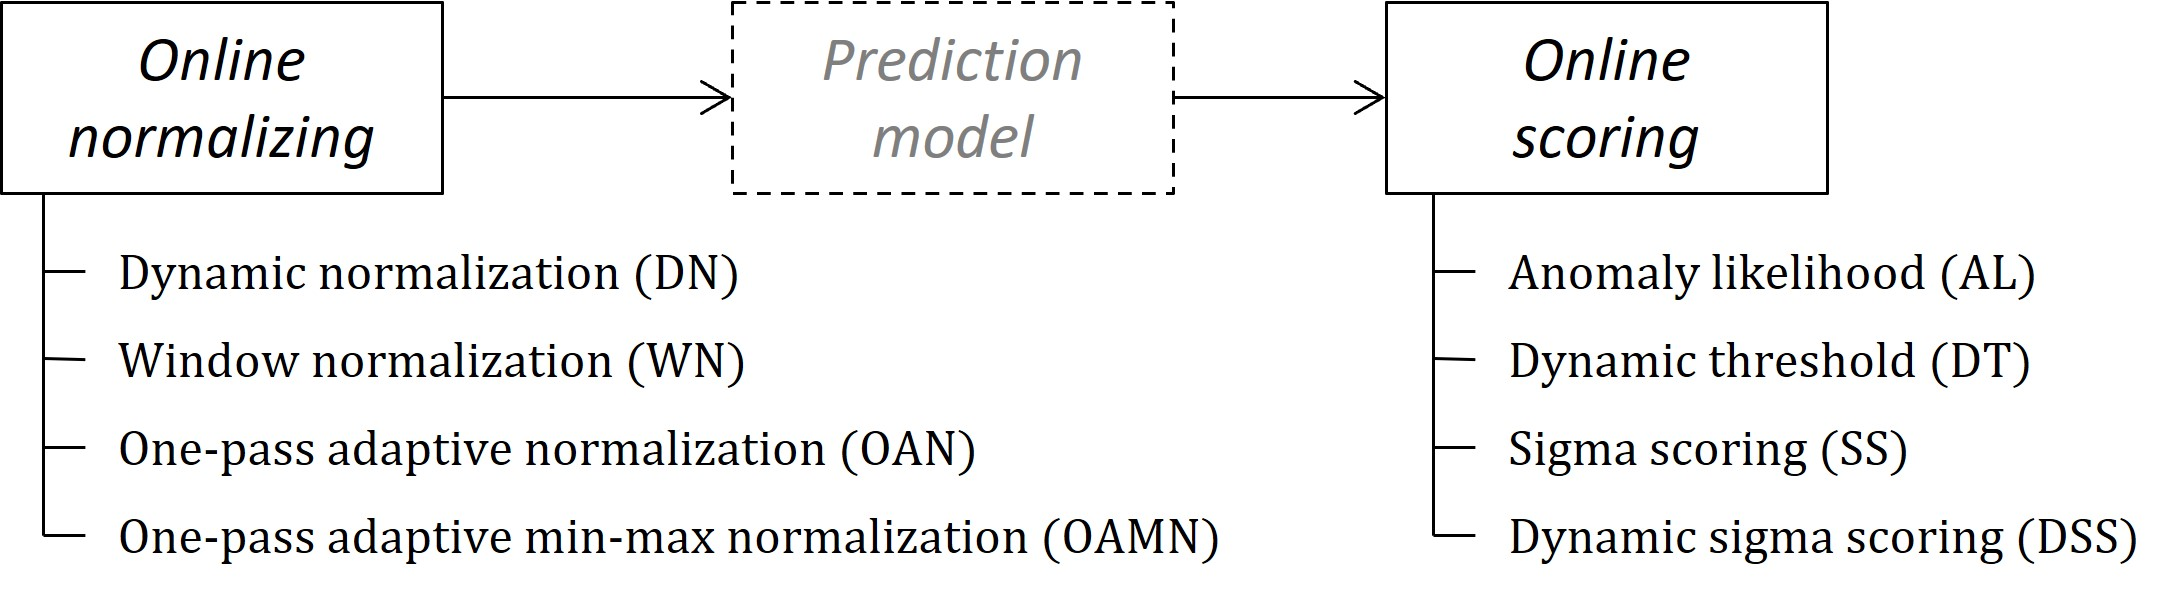
\includegraphics[width=0.5\linewidth]{AD-FRAMEWORK.jpg}
\caption{Procedure to adapt online prediction models to outlier detection using the proposed framework.}
\label{fig:ad-framework}
\end{figure}

In Figure \ref{fig:ad-framework}, in addition to the procedure for transforming a prediction algorithm into an anomaly detection algorithm, the normalization and scoring functions contained in each component are also shown.

\subsubsection{Online normalization component}

\begin{itemize}

\item \emph{DN} or \emph{Dynamic nomalization}. This method is introduced by Bollegala \cite{Bollegala2017}. In there, the classical z-score standardization Eq. \eqref{eq:z-score} is applied using dynamically calculated mean Eq. \eqref{eq:dynamic-mean} and deviation Eq. (\ref{eq:dynamic-s}).

\begin{equation}\label{eq:z-score}
    x' = \frac{x - \mu}{\sigma}
\end{equation}

\begin{equation} \label{eq:dynamic-mean}
    \mu_{t} = \mu_{t-1} + \frac{x_{t} - \mu_{t-1}}{t}
\end{equation}

\begin{equation} \begin{aligned} \label{eq:dynamic-s}
    s_{t} &= s_{t-1} + (x_{t} - \mu_{t-1})(x_{t} - \mu_{t}) \\
    \sigma_{t} &= \sqrt{s_{t} / (t-1)}
\end{aligned} \end{equation}

\item \emph{WN} or \emph{Window nomalization}. This is the traditional approach, used by  Lin and Keogh \cite{Lin2004} and Haykin  \cite{haykin2009neural}, that consists of dividing time series into sliding windows $W$ first, and then normalizing or standardizing them according to the statistical properties ($\mu$ and $\sigma$) inferred from the last window $W$. In one-pass normalization, a sliding window $W$ is updated with the last $n$ data instances whenever a new data $x_{t}$ arrives, i.e.,  $W = \{x_{t-n+1}, ..., x_{t}\}$. Then, considering the statics of the sliding window $W$, the whole $W$ (or only the current data instance $x_{t}$) is normalized.

\item \emph{OAN} or \emph{One-pass adaptive nomalization}. This is our adaptation for one-pass learning of the adaptive normalization introduced by Ogasawara et al. \cite{Ogasawara2010}. This method is specifically designed to normalize non-stationary heteroscedastic (non-uniform volatility) time series and is used for neural network learning. Furthermore, it is important to note that the original method is not fully incremental since it is used to train different neural networks (NN) offline. However, it presents some incremental properties, which we exploit to its application in an online environment.

\item \emph{OAMN} or \emph{One-pass adaptive min-max nomalization}. This is a one-pass adaptation of the adaptive min-max normalization for Big Data stream proposed by Gupta and Hewett \cite{Gupta2019}. The original proposal was designed for online chunk-by-chunk (batches of data) processing, where disjoint (non-overlapping) fixed size sliding windows $W_{i}$ are used. In this case, one-pass overlapping windows are used.

\end{itemize}

\subsubsection{Online outlier scoring component}

\begin{itemize}

\item \emph{AL} or \emph{Anomaly likelihood}. This is a novel incremental thresholding approach introduced by Ahamd et al. in \cite{Ahmad2017} and used along with the Hierarchical Temporal Memory (HTM) prediction algorithm to provide the HTM anomaly detector. Anomaly likelihood is a generalist method completely independent from the prediction model, which only needs the prediction errors.
\item \emph{DT} or \emph{Dynamic threshold}. This method was introduced by Buda et al. \cite{Buda2018} and computes the dynamic threshold based on a sliding window of historical normalized prediction errors that are labeled as inliner. The dynamic threshold is calculated as ten times the standard deviation of the historical window. An anomaly is reported if the normalized current error value is equal to or bigger than the dynamic threshold.
\item \emph{SS} or \emph{Sigma scoring}. This is our online scoring proposal based on 3-sigma control charts and the scoring method proposed in \cite{Wang2019},  originally used to score the anomalies detected by One-Class based outlier detectors. In order to adapt this scoring method to online 3-sigma control limits, the radius is defined as $R = 3\sigma_{t}$ and the center as $o = \mu_{t}$; where $\sigma_{t}$ and $\mu_{t}$ are the standard deviation and the mean of the current window $W_{t}$. Hence, this method fulfills these desirable four criteria:

    \begin{itemize}
        \item [(1)] $0 < score(x) < 1$
        \item [(2)] $score(x) = 0.5$ for samples on the boundary
        \item [(3)] $score(x) < 0.5$ for samples inside the boundary
        \item [(4)] $score(x) > 0.5$ for samples outside the boundary
    \end{itemize}

\item \emph{DSS} or \emph{Dynamic sigma scoring}. This is a dynamic version of the previous SS method. In this case, the mean and the standard deviation are computed dynamically whenever a new prediction error arrives instead of a sliding window. The dynamic mean $\mu_{t}$, and dynamic standard deviation $\sigma_{t}$ are computed using the Eq. \eqref{eq:dynamic-mean} and Eq. \eqref{eq:dynamic-s} proposed in \cite{Bollegala2017} for dynamic data normalization.

\end{itemize}


\section{Use example}\label{sec:examplesec}

In this section we explain how to use the package. Section \ref{sec:installation} describes  how to install the package. In section \ref{sec:documentation} we show how to load the documentation. Then, section \ref{sec:examples} includes some examples to show how to use the package. Finally, section \ref{sec:summaryfunctions} summarizes the most useful functions.

\subsection{Installation}\label{sec:installation}

The \pkg{otsad} package is available at GitHub repository, so it can be downloaded and installed directly from the R command line by typing:

\begin{knitrout}
\definecolor{shadecolor}{rgb}{0.969, 0.969, 0.969}\color{fgcolor}\begin{kframe}
\begin{alltt}
\hlkwd{install.packages}\hlstd{(}\hlstr{"devtools"}\hlstd{)}
\hlstd{devtools}\hlopt{::}\hlkwd{install_github}\hlstd{(}\hlstr{"alaineiturria/otsad"}\hlstd{)}
\end{alltt}
\end{kframe}
\end{knitrout}

To easily access all the package’s functions, it must be attached in the usual way:

\begin{knitrout}
\definecolor{shadecolor}{rgb}{0.969, 0.969, 0.969}\color{fgcolor}\begin{kframe}
\begin{alltt}
\hlkwd{library}\hlstd{(otsad)}
\end{alltt}
\end{kframe}
\end{knitrout}

\textbf{Special note: }

CAD-OSE executes a python script so it is necessary to have python2 or python3 installed. In addition, to get the same results in all operating systems it is necessary to have installed the hashlib and bencode-python3 python libraries.

\subsection{Documentation}\label{sec:documentation}

Considering that this vignette provides the user with an overview of the \pkg{otsad} package, it is also important to have access to the specific information of each of the available algorithms. This information can be checked in the documentation page corresponding to each algorithm. In all cases, the documentation has the same structure, consisting of the following sections (see Figure \ref{fig:documentation} for an example):

\begin{itemize}
\item A \emph{description} section, which gives a brief description of what the algorithm consists of (like those given in Section \ref{sec:package}).
\item A \emph{usage} section, where an overview of the function with the available parameters is given.
\item An \emph{arguments} section, where each of the input parameters is described.
\item A \emph{details} section, which provides the user with more details on the algorithm, conditions and recommendations on the values that can be taken by each of the input parameters.
\item A \emph{value} section, where the output parameters of the function are described.
\item A \emph{references} section that points to the original contribution where the detector(s) was proposed, where further details, motivations or contextualization can be found.
\item An \emph{examples} section, where one or more examples of the use of the functions are shown.
\end{itemize}

As usual in R, the documentation pages for each function can be loaded from the command line with the commands \code{?} or \code{help}:

\begin{knitrout}
\definecolor{shadecolor}{rgb}{0.969, 0.969, 0.969}\color{fgcolor}\begin{kframe}
\begin{alltt}
\hlopt{?}\hlstd{CpSdEwma}
\hlkwd{help}\hlstd{(CpSdEwma)}
\end{alltt}
\end{kframe}
\end{knitrout}

In addition, a user manual is available in the github repository of the  \pkg{otsad} package, which contains the complete documentation of the package and its functions.

\begin{figure}[htbp]
\centering
\includegraphics[width=0.5\linewidth]{documentationExample.png}
\caption{Extract from CpSdEwma detectors documentation page, showing the highlighted above aspects.}
\label{fig:documentation}
\end{figure}

\newpage

\subsection{Examples}\label{sec:examples}

For the sake of clarity we have divided the examples into three blocks. In Section \ref{sec:examples-bloq1} we introduce how to detect anomalies and visualize the results. Then Section \label{sec:examples-bloq2} introduces how to measure anomaly detectors. Finally, in Section \label{sec:examples-bloq3} we show an example of using the framework to adapt a prediction algorithm to outlier detection.

\subsubsection{Anomaly detection and visualization}\label{sec:examples-bloq1}

\begin{itemize}

 \item \textbf{Example 1:} \textit{How to solve a simple problem using SD-EWMA algorithm.}

  The data has been generated as follows:

\begin{knitrout}
\definecolor{shadecolor}{rgb}{0.969, 0.969, 0.969}\color{fgcolor}\begin{kframe}
\begin{alltt}
\hlcom{## Generate data}
\hlkwd{set.seed}\hlstd{(}\hlnum{100}\hlstd{)}
\hlstd{n} \hlkwb{<-} \hlnum{500}
\hlstd{x} \hlkwb{<-} \hlkwd{sample}\hlstd{(}\hlnum{1}\hlopt{:}\hlnum{100}\hlstd{, n,} \hlkwc{replace} \hlstd{=} \hlnum{TRUE}\hlstd{)}
\hlstd{x[}\hlnum{70}\hlopt{:}\hlnum{90}\hlstd{]} \hlkwb{<-} \hlkwd{sample}\hlstd{(}\hlnum{110}\hlopt{:}\hlnum{115}\hlstd{,} \hlnum{21}\hlstd{,} \hlkwc{replace} \hlstd{=} \hlnum{TRUE}\hlstd{)} \hlcom{# distributional shift}
\hlstd{x[}\hlnum{25}\hlstd{]} \hlkwb{<-} \hlnum{200} \hlcom{# abrupt transient anomaly}
\hlstd{x[}\hlnum{320}\hlstd{]} \hlkwb{<-} \hlnum{170} \hlcom{# abrupt transient anomaly}
\hlstd{df} \hlkwb{<-} \hlkwd{data.frame}\hlstd{(}\hlkwc{timestamp} \hlstd{=} \hlnum{1}\hlopt{:}\hlstd{n,} \hlkwc{value} \hlstd{= x)}
\end{alltt}
\end{kframe}
\end{knitrout}

  We can visualize the time-series as in Figure \ref{fig:ts} by typing:
\begin{knitrout}
\definecolor{shadecolor}{rgb}{0.969, 0.969, 0.969}\color{fgcolor}\begin{kframe}
\begin{alltt}
\hlkwd{plot}\hlstd{(}\hlkwc{x} \hlstd{= df}\hlopt{$}\hlstd{timestamp,} \hlkwc{y} \hlstd{= df}\hlopt{$}\hlstd{value,} \hlkwc{type} \hlstd{=} \hlstr{"l"}\hlstd{,}
     \hlkwc{main} \hlstd{=} \hlstr{"Time-Serie"}\hlstd{,} \hlkwc{col} \hlstd{=} \hlstr{"blue"}\hlstd{,} \hlkwc{xlab} \hlstd{=} \hlstr{"Time"}\hlstd{,} \hlkwc{ylab} \hlstd{=} \hlstr{"Value"}\hlstd{)}
\end{alltt}
\end{kframe}
\end{knitrout}

  \begin{figure}[htbp]
  \centering
  \includegraphics[width=0.7\linewidth]{timeSerie.png}
  \caption{Our time-series visualization}
  \label{fig:ts}
  \end{figure}


  The SD-EWMA algorithm is designed for stationary time-series. Therefore, we must first check that the time-series is stationary. To do this, we can display the acf and pacf graphics (Figure \ref{fig:acf}) by:

\begin{knitrout}
\definecolor{shadecolor}{rgb}{0.969, 0.969, 0.969}\color{fgcolor}\begin{kframe}
\begin{alltt}
\hlstd{forecast}\hlopt{::}\hlkwd{Acf}\hlstd{(}\hlkwd{ts}\hlstd{(df}\hlopt{$}\hlstd{value),} \hlkwc{main} \hlstd{=} \hlstr{"ACF"}\hlstd{,} \hlkwc{lag} \hlstd{=} \hlnum{20}\hlstd{)}
\hlstd{forecast}\hlopt{::}\hlkwd{Pacf}\hlstd{(}\hlkwd{ts}\hlstd{(df}\hlopt{$}\hlstd{value),} \hlkwc{main} \hlstd{=} \hlstr{"PACF"}\hlstd{,} \hlkwc{lag} \hlstd{=} \hlnum{20}\hlstd{)}
\end{alltt}
\end{kframe}
\end{knitrout}

  \begin{figure}[htbp]
  \centering
  \includegraphics[width=0.7\linewidth]{acf.png}
  \caption{ACF and PACF graphs}
  \label{fig:acf}
  \end{figure}

  We can observe that since almost all the lags are within the limits, the time-series is stationary. In addition, we can use two statistical tests, adf test and kpss test. The tests also indicate that the time-series is stationary.

\begin{knitrout}
\definecolor{shadecolor}{rgb}{0.969, 0.969, 0.969}\color{fgcolor}\begin{kframe}
\begin{alltt}
\hlkwd{library}\hlstd{(tseries)}
\hlkwd{adf.test}\hlstd{(df}\hlopt{$}\hlstd{value,} \hlkwc{alternative} \hlstd{=} \hlstr{'stationary'}\hlstd{,} \hlkwc{k} \hlstd{=} \hlnum{0}\hlstd{)}
\hlkwd{kpss.test}\hlstd{(df}\hlopt{$}\hlstd{value)}
\end{alltt}
\end{kframe}
\end{knitrout}

  On the recommendation of the algorithm authors we set \code{threshold} to 0.01.One of the usual values for the $\sigma$ multiplier \code{l} is usually 3. Next, we apply the SD-EWMA anomaly detector, as the example is simple we use the classical processing algorithm. Note that the optimized algorithm could be used in the same way. Finally, we separate the training and test sets, using the first five values for training and the rest values for testing.

\begin{knitrout}
\definecolor{shadecolor}{rgb}{0.969, 0.969, 0.969}\color{fgcolor}\begin{kframe}
\begin{alltt}
\hlstd{result} \hlkwb{<-} \hlkwd{CpSdEwma}\hlstd{(}\hlkwc{data} \hlstd{= df}\hlopt{$}\hlstd{value,} \hlkwc{n.train} \hlstd{=} \hlnum{5}\hlstd{,} \hlkwc{threshold} \hlstd{=} \hlnum{0.01}\hlstd{,} \hlkwc{l} \hlstd{=} \hlnum{3}\hlstd{)}
\end{alltt}
\end{kframe}
\end{knitrout}

  This results are of data.frame type and have three columns: \emph{is.anomaly} indicating whether or not the test observation is anomalous and the columns \emph{ucl} and \emph{lcl} with the upper and lower control limits, used to determine whether or not the observation is anomalous.

\begin{knitrout}
\definecolor{shadecolor}{rgb}{0.969, 0.969, 0.969}\color{fgcolor}\begin{kframe}
\begin{alltt}
\hlkwd{head}\hlstd{(result,} \hlkwc{n} \hlstd{=} \hlnum{15}\hlstd{)}
\end{alltt}
\begin{verbatim}
##    is.anomaly         lcl      ucl
## 1           0  74.0000000  74.0000
## 2           0  89.0000000  89.0000
## 3           0  78.0000000  78.0000
## 4           0  23.0000000  23.0000
## 5           0  86.0000000  86.0000
## 6           0   0.2998149 139.0313
## 7           0   0.6808881 138.7171
## 8           0  -8.3155413 134.5737
## 9           0  -8.8121491 133.4445
## 10          0  -7.7247629 133.8939
## 11          0  -4.6526720 137.8049
## 12          0 -12.4721436 133.7091
## 13          0 -19.2253248 129.7386
## 14          0 -18.8776837 129.3396
## 15          0 -19.8205462 127.8363
\end{verbatim}
\end{kframe}
\end{knitrout}

  Finally, we can plot the results (Figure \ref{fig:result}) by writing the following code:

\begin{knitrout}
\definecolor{shadecolor}{rgb}{0.969, 0.969, 0.969}\color{fgcolor}\begin{kframe}
\begin{alltt}
\hlstd{res} \hlkwb{<-} \hlkwd{cbind}\hlstd{(df, result)}
\hlkwd{PlotDetections}\hlstd{(res,} \hlkwc{title} \hlstd{=} \hlstr{"SD-EWMA ANOMALY DETECTOR"}\hlstd{)}
\end{alltt}
\end{kframe}
\end{knitrout}

  \begin{figure}[htbp]
  \centering
  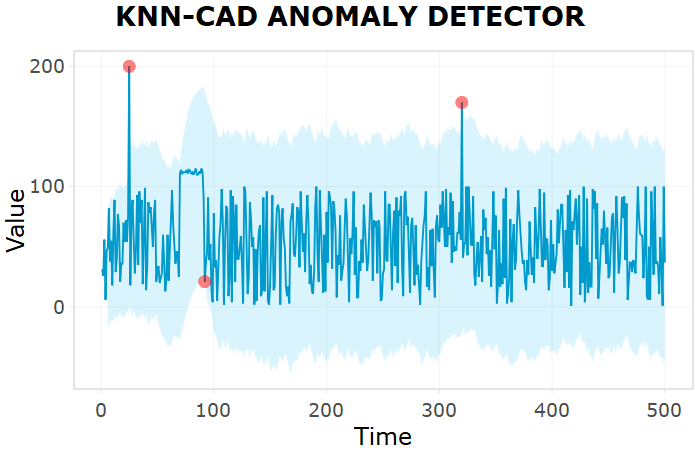
\includegraphics[width=0.5\linewidth]{sdEwmaresult.png}
  \caption{Sd-Ewma Anomaly detector results}
  \label{fig:result}
  \end{figure}

  In Figure \ref{fig:result} we can see that the detector has detected well both abrupt transient anomalies  and distributional shift anomaly.

  This example has used classical processing, but by using the incremental function we can simulate online processing as follows:

\begin{knitrout}
\definecolor{shadecolor}{rgb}{0.969, 0.969, 0.969}\color{fgcolor}\begin{kframe}
\begin{alltt}
\hlcom{## Initialize parameters for the loop}
\hlstd{last.res} \hlkwb{<-} \hlkwa{NULL}
\hlstd{res} \hlkwb{<-} \hlkwa{NULL}
\hlstd{nread} \hlkwb{<-} \hlnum{250}
\hlstd{numIter} \hlkwb{<-} \hlstd{n}\hlopt\hlstd{nread}
\hlstd{iter} \hlkwb{<-} \hlkwd{seq}\hlstd{(}\hlnum{1}\hlstd{, nread} \hlopt{*} \hlstd{numIter, nread)}

\hlcom{## Calculate anomalies}
\hlkwa{for}\hlstd{(i} \hlkwa{in} \hlstd{iter) \{}
  \hlcom{# read new data}
  \hlstd{newRow} \hlkwb{<-} \hlstd{df[i}\hlopt{:}\hlstd{(i} \hlopt{+} \hlstd{nread} \hlopt{-} \hlnum{1}\hlstd{),]}
  \hlcom{# calculate if it's an anomaly}
  \hlstd{last.res} \hlkwb{<-} \hlkwd{IpSdEwma}\hlstd{(}
    \hlkwc{data} \hlstd{= newRow}\hlopt{$}\hlstd{value,}
    \hlkwc{n.train} \hlstd{=} \hlnum{5}\hlstd{,}
    \hlkwc{threshold} \hlstd{=} \hlnum{0.01}\hlstd{,}
    \hlkwc{l} \hlstd{=} \hlnum{3}\hlstd{,}
    \hlkwc{last.res} \hlstd{= last.res}\hlopt{$}\hlstd{last.res}
  \hlstd{)}
  \hlcom{# prepare the result}
  \hlkwa{if}\hlstd{(}\hlopt{!}\hlkwd{is.null}\hlstd{(last.res}\hlopt{$}\hlstd{result))\{}
    \hlstd{res} \hlkwb{<-} \hlkwd{rbind}\hlstd{(res,} \hlkwd{cbind}\hlstd{(newRow, last.res}\hlopt{$}\hlstd{result))}
  \hlstd{\}}
\hlstd{\}}
\end{alltt}
\end{kframe}
\end{knitrout}

  In the same way we can plot the results (Figure ref{fig:result2}) by writing:

\begin{knitrout}
\definecolor{shadecolor}{rgb}{0.969, 0.969, 0.969}\color{fgcolor}\begin{kframe}
\begin{alltt}
\hlkwd{PlotDetections}\hlstd{(res,} \hlkwc{title} \hlstd{=} \hlstr{"SD-EWMA ANOMALY DETECTOR"}\hlstd{)}
\end{alltt}
\end{kframe}
\end{knitrout}

  \begin{figure}[htbp]
  \centering
  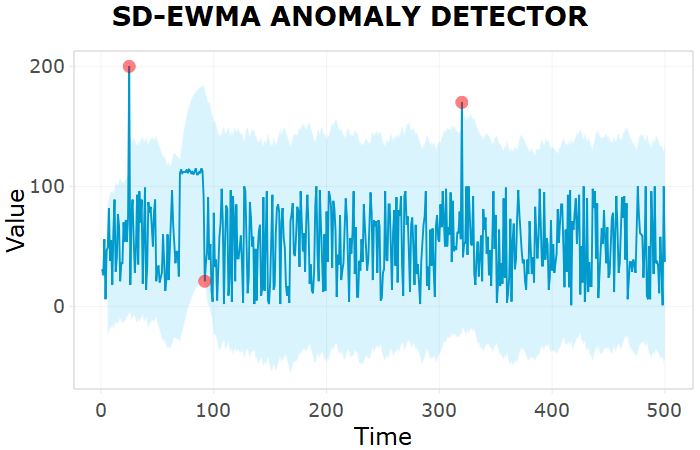
\includegraphics[width=0.5\linewidth]{onlineSdEwma.png}
  \caption{Online Sd-Ewma Anomaly detector results}
  \label{fig:result2}
  \end{figure}

  \item \textbf{Example 2:} \textit{How to use Contextual Anomaly Detector.} The use of the Contextual Anomaly Detector is similar to the use of the previous algorithm. It is important to note that if the bencode python module is not installed, this method will rise an error. This can be prevented installing the bencode-pyhthon3 library with Python package manager \code{pip}.

\begin{knitrout}
\definecolor{shadecolor}{rgb}{0.969, 0.969, 0.969}\color{fgcolor}\begin{kframe}
\begin{alltt}
\hlstd{cad.results} \hlkwb{<-} \hlkwd{ContextualAnomalyDetector}\hlstd{(}
  \hlstd{df}\hlopt{$}\hlstd{value[}\hlnum{1}\hlopt{:}\hlnum{250}\hlstd{],}
  \hlkwc{base.threshold} \hlstd{=} \hlnum{0.75}\hlstd{,}
  \hlkwc{rest.period} \hlstd{=} \hlnum{5}\hlstd{,}
  \hlkwc{max.value} \hlstd{=} \hlnum{200}\hlstd{,}
  \hlkwc{min.value} \hlstd{=} \hlnum{0}
\hlstd{)}
\hlstd{cad.results.online} \hlkwb{<-} \hlkwd{ContextualAnomalyDetector}\hlstd{(}
  \hlstd{df}\hlopt{$}\hlstd{value[}\hlnum{251}\hlopt{:}\hlnum{500}\hlstd{],}
  \hlkwc{python.object} \hlstd{= cad.results}\hlopt{$}\hlstd{python.Object}
\hlstd{)}

\hlstd{res} \hlkwb{<-} \hlkwd{cbind}\hlstd{(df,} \hlkwd{rbind}\hlstd{(cad.results}\hlopt{$}\hlstd{result, cad.results.online}\hlopt{$}\hlstd{result))}
\hlkwd{PlotDetections}\hlstd{(res,} \hlkwc{title} \hlstd{=} \hlstr{"CONTEXTUAL ANOMALY DETECTOR"}\hlstd{)}
\end{alltt}
\end{kframe}
\end{knitrout}

  \begin{figure}[htbp]
  \centering
  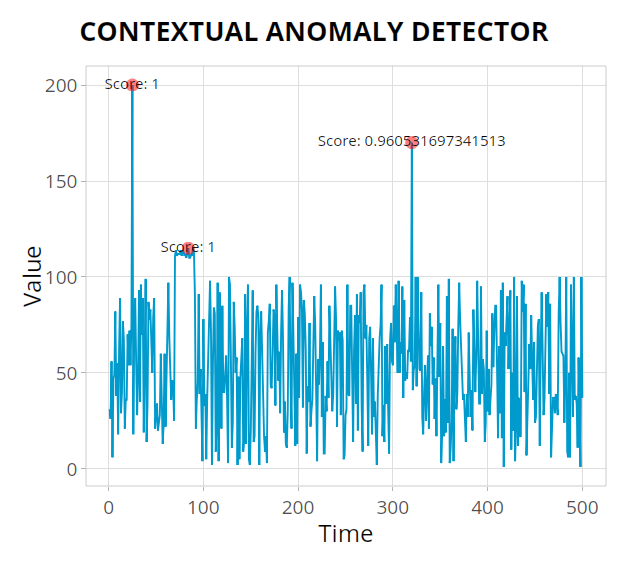
\includegraphics[width=0.5\linewidth]{cadose.png}
  \caption{Contextual Anomaly Detector results}
  \label{fig:cad}
  \end{figure}

  \item \textbf{Example 3:} \textit{How to use EORELM-AD.} The use of the EORELM-AD algorithm is quite like the use of previous algorithms. However, for its easier use, it is implemented as an R6 class. Because of that, unlike the other algorithms, first, the EorelmAD object must be created as follow.

\begin{knitrout}
\definecolor{shadecolor}{rgb}{0.969, 0.969, 0.969}\color{fgcolor}\begin{kframe}
\begin{alltt}
\hlstd{detector} \hlkwb{<-} \hlstd{EorelmAD}\hlopt{$}\hlkwd{new}\hlstd{(}
  \hlkwc{n.train} \hlstd{=} \hlnum{20}\hlstd{,}
  \hlkwc{numLags} \hlstd{=} \hlnum{10}\hlstd{,}
  \hlkwc{numHiddenNeurons} \hlstd{=} \hlkwd{c}\hlstd{(}\hlnum{20}\hlstd{),}
  \hlkwc{normMethod} \hlstd{=} \hlkwa{NULL}\hlstd{,}
  \hlkwc{outlierMethod} \hlstd{=} \hlstr{"DSS"}\hlstd{,}
  \hlkwc{threshold} \hlstd{=} \hlnum{0.5}
\hlstd{)}
\end{alltt}
\end{kframe}
\end{knitrout}

  Now the anomaly detection is carried out. To do this, the prediction method is used. As an argument, it takes a single value or a set of values in which anomalies should be detected. In this case, the whole dataset is used.
\begin{knitrout}
\definecolor{shadecolor}{rgb}{0.969, 0.969, 0.969}\color{fgcolor}\begin{kframe}
\begin{alltt}
\hlstd{result} \hlkwb{<-} \hlstd{detector}\hlopt{$}\hlkwd{predict}\hlstd{(df}\hlopt{$}\hlstd{value)}

\hlcom{## Plot results}
\hlstd{res} \hlkwb{<-} \hlkwd{cbind}\hlstd{(df, result)}
\hlkwd{PlotDetections}\hlstd{(res,} \hlkwc{title} \hlstd{=} \hlstr{"EORELM-AD ANOMALY DETECTOR"}\hlstd{,} \hlkwc{return.ggplot} \hlstd{=} \hlnum{TRUE}\hlstd{)}
\end{alltt}
\end{kframe}
\end{knitrout}

  \begin{figure}[htbp]
  \centering
  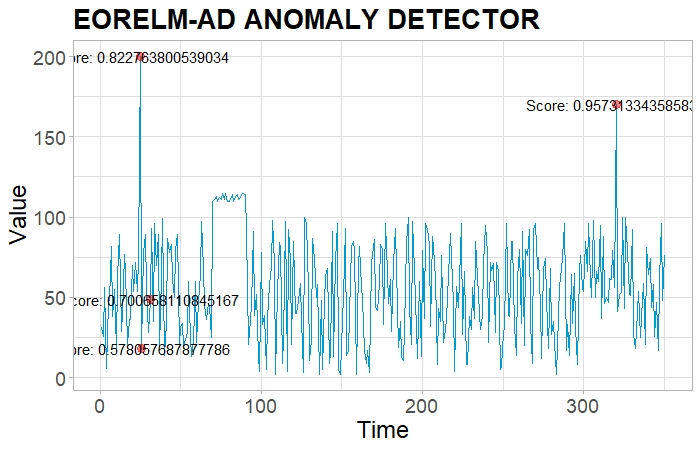
\includegraphics[width=0.5\linewidth]{eorelm_ad_result.jpeg}
  \caption{EORELM-AD results}
  \label{fig:eorelm-res}
  \end{figure}

  \item \textbf{Example 4:} \textit{How to use KNN.} In this example KNN is used to detect the five anomalies of the \emph{Speed\_7578} dataset.

\begin{knitrout}
\definecolor{shadecolor}{rgb}{0.969, 0.969, 0.969}\color{fgcolor}\begin{kframe}
\begin{alltt}
\hlcom{# Load the previously installed otsad package}
\hlkwd{library}\hlstd{(}\hlstr{"otsad"}\hlstd{)}

\hlcom{# Load the dataset speed_7578, included in otsad}
\hlstd{myData} \hlkwb{<-} \hlstd{speed_7578}

\hlcom{# Initialize parameters}
\hlstd{n} \hlkwb{<-} \hlkwd{nrow}\hlstd{(myData)}
\hlstd{n.train} \hlkwb{<-} \hlkwd{GetNumTrainingValues}\hlstd{(n)}

\hlcom{# Calculate anomalies using KNN-CAD}
\hlstd{result} \hlkwb{<-} \hlkwd{CpKnnCad}\hlstd{(}
  \hlkwc{data} \hlstd{= myData}\hlopt{$}\hlstd{value,}
  \hlkwc{n.train} \hlstd{= n.train,}
  \hlkwc{threshold} \hlstd{=} \hlnum{1}\hlstd{,}
  \hlkwc{l} \hlstd{=} \hlnum{19}\hlstd{,}
  \hlkwc{k} \hlstd{=} \hlnum{27}\hlstd{,}
  \hlkwc{ncm.type} \hlstd{=} \hlstr{"ICAD"}\hlstd{,}
  \hlkwc{reducefp} \hlstd{=} \hlnum{TRUE}
\hlstd{)}

\hlcom{# Add results to dataset}
\hlstd{myData} \hlkwb{<-} \hlkwd{cbind}\hlstd{(myData, result)}
\end{alltt}
\end{kframe}
\end{knitrout}

  Once the algorithm is applied, we could show the results using the PlotDetections function. Since the resulting graph is interactive, in Figure \ref{fig:Example1Score} we show a capture of it.

\begin{knitrout}
\definecolor{shadecolor}{rgb}{0.969, 0.969, 0.969}\color{fgcolor}\begin{kframe}
\begin{alltt}
\hlcom{# Plot Results}
\hlkwd{PlotDetections}\hlstd{(myData,} \hlkwc{title} \hlstd{=} \hlstr{"KNN-CAD ANOMALY DETECTOR"}\hlstd{)}
\end{alltt}
\end{kframe}
\end{knitrout}

  \begin{figure}[htbp]
  \centering
  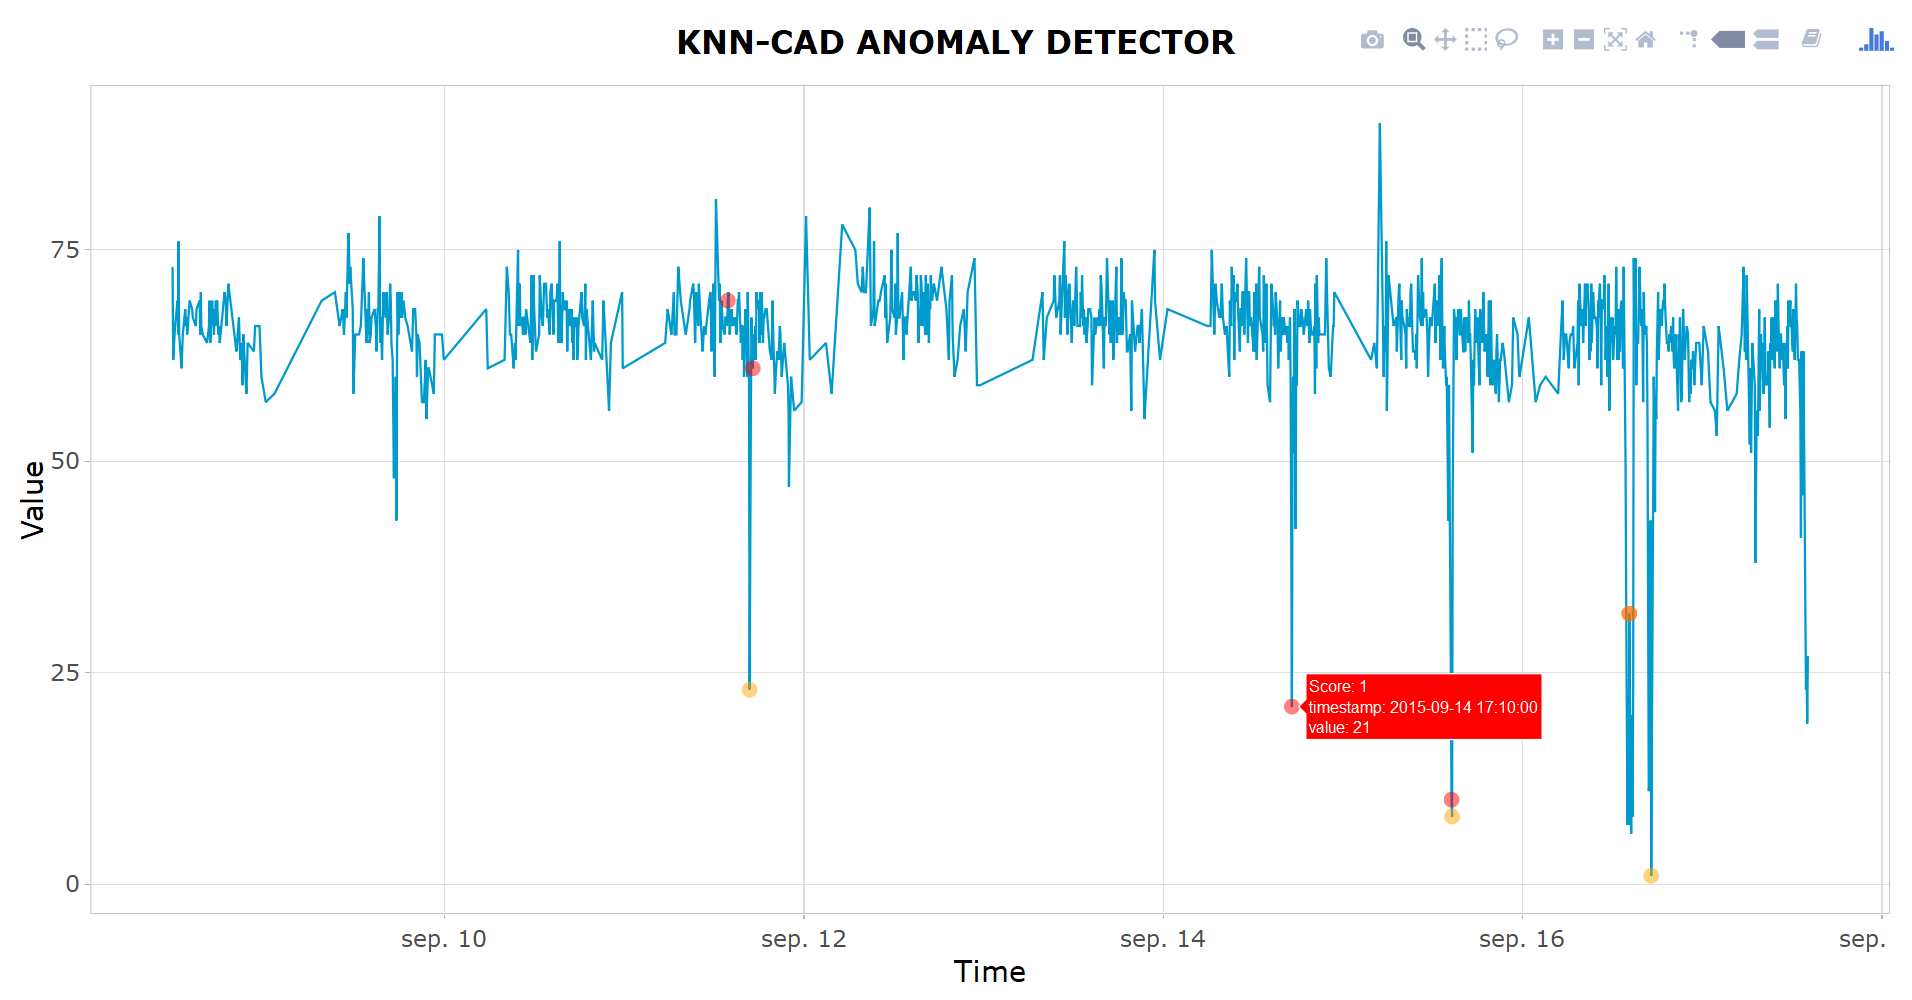
\includegraphics[width=1\linewidth]{Example1Score.png}
  \caption{Anomalies detected in speed\_7578 dataset by KNN\_CAD detector.}
  \label{fig:Example1Score}
  \end{figure}

\end{itemize}

\subsubsection{Detector measuerement}\label{sec:examples-bloq2}

  Example 4 is continued to show how to measure the performance of the detector.
  Hence, the detector's score is obtained as follow:

\begin{knitrout}
\definecolor{shadecolor}{rgb}{0.969, 0.969, 0.969}\color{fgcolor}\begin{kframe}
\begin{alltt}
\hlcom{# Get detector score}
\hlstd{score} \hlkwb{<-} \hlkwd{GetDetectorScore}\hlstd{(myData)}

\hlcom{# See this results}
\hlkwd{data.frame}\hlstd{(score[}\hlopt{-}\hlnum{1}\hlstd{])}
\end{alltt}
\end{kframe}
\end{knitrout}

  This function has an option to show the results on a chart by adding the following parameters, see \ref{fig:Ej1ScoreDe}.

\begin{knitrout}
\definecolor{shadecolor}{rgb}{0.969, 0.969, 0.969}\color{fgcolor}\begin{kframe}
\begin{alltt}
\hlcom{# Get detector score}
\hlstd{score} \hlkwb{<-} \hlkwd{GetDetectorScore}\hlstd{(}
  \hlstd{myData,}
  \hlkwc{print} \hlstd{=} \hlnum{TRUE}\hlstd{,}
  \hlkwc{title} \hlstd{=} \hlstr{"speed_7578 results using KNN-CAD detector"}
\hlstd{)}
\end{alltt}
\end{kframe}
\end{knitrout}

  \begin{figure}[htbp]
  \centering
  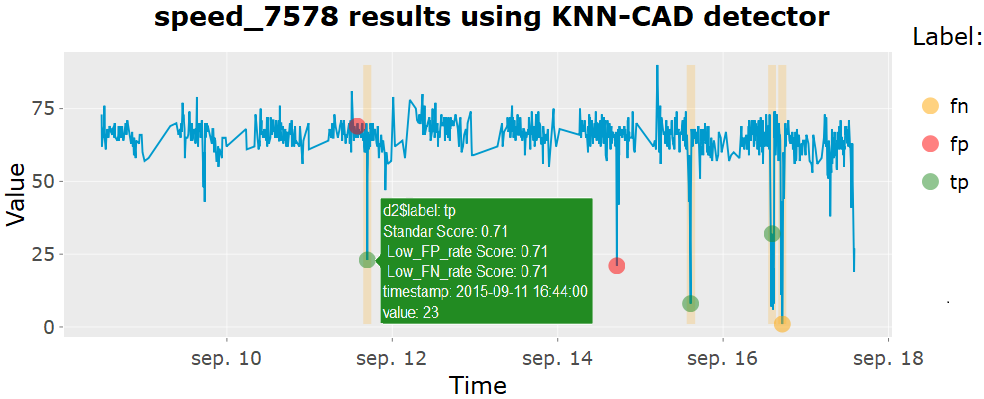
\includegraphics[width=1\linewidth]{Ej1ScoreDe.png}
  \caption{KNN-CAD detector measurement results for speed\_7578 dataset.}
  \label{fig:Ej1ScoreDe}
  \end{figure}

  Finally, we normalize the scores and show them.

\begin{knitrout}
\definecolor{shadecolor}{rgb}{0.969, 0.969, 0.969}\color{fgcolor}\begin{kframe}
\begin{alltt}
\hlcom{# Normalize results}
\hlstd{null.perfect} \hlkwb{<-} \hlkwd{GetNullAndPerfectScores}\hlstd{(myData)}

\hlstd{standar.score} \hlkwb{<-} \hlkwd{NormalizeScore}\hlstd{(}
  \hlstd{score}\hlopt{$}\hlstd{standard,}
  \hlkwc{perfect.score} \hlstd{= null.perfect[}\hlnum{1}\hlstd{,} \hlstr{"perfect.score"}\hlstd{],}
  \hlkwc{null.score} \hlstd{= null.perfect[}\hlnum{1}\hlstd{,} \hlstr{"null.score"}\hlstd{]}
\hlstd{)}

\hlstd{low_FP_rate.score} \hlkwb{<-} \hlkwd{NormalizeScore}\hlstd{(}
  \hlstd{score}\hlopt{$}\hlstd{low_FP_rate,}
  \hlkwc{perfect.score} \hlstd{= null.perfect[}\hlnum{2}\hlstd{,} \hlstr{"perfect.score"}\hlstd{],}
  \hlkwc{null.score} \hlstd{= null.perfect[}\hlnum{2}\hlstd{,} \hlstr{"null.score"}\hlstd{]}
\hlstd{)}

\hlstd{low_FN_rate.score} \hlkwb{<-} \hlkwd{NormalizeScore}\hlstd{(}
  \hlstd{score}\hlopt{$}\hlstd{low_FN_rate,}
  \hlkwc{perfect.score} \hlstd{= null.perfect[}\hlnum{3}\hlstd{,} \hlstr{"perfect.score"}\hlstd{],}
  \hlkwc{null.score} \hlstd{= null.perfect[}\hlnum{3}\hlstd{,} \hlstr{"null.score"}\hlstd{]}
\hlstd{)}

\hlcom{# Show normalized scores}
\hlkwd{cbind}\hlstd{(standar.score, low_FP_rate.score, low_FN_rate.score)}
\end{alltt}
\end{kframe}
\end{knitrout}

\subsubsection{Adapting prediction algorithm to anomaly detection}\label{sec:examples-bloq3}

The data set used for this example is the following one:

\begin{knitrout}
\definecolor{shadecolor}{rgb}{0.969, 0.969, 0.969}\color{fgcolor}\begin{kframe}
\begin{alltt}
\hlcom{## Generate data}
\hlkwd{set.seed}\hlstd{(}\hlnum{100}\hlstd{)}
\hlstd{n} \hlkwb{<-} \hlnum{500}
\hlstd{x} \hlkwb{<-} \hlkwd{sample}\hlstd{(}\hlnum{1}\hlopt{:}\hlnum{100}\hlstd{, n,} \hlkwc{replace} \hlstd{=} \hlnum{TRUE}\hlstd{)}
\hlstd{x[}\hlnum{70}\hlopt{:}\hlnum{90}\hlstd{]} \hlkwb{<-} \hlkwd{sample}\hlstd{(}\hlnum{110}\hlopt{:}\hlnum{115}\hlstd{,} \hlnum{21}\hlstd{,} \hlkwc{replace} \hlstd{=} \hlnum{TRUE}\hlstd{)} \hlcom{# distributional shift}
\hlstd{x[}\hlnum{25}\hlstd{]} \hlkwb{<-} \hlnum{200} \hlcom{# abrupt transient anomaly}
\hlstd{x[}\hlnum{320}\hlstd{]} \hlkwb{<-} \hlnum{170} \hlcom{# abrupt transient anomaly}
\hlstd{df} \hlkwb{<-} \hlkwd{data.frame}\hlstd{(}\hlkwc{timestamp} \hlstd{=} \hlnum{1}\hlopt{:}\hlstd{n,} \hlkwc{value} \hlstd{= x)}
\end{alltt}
\end{kframe}
\end{knitrout}

Now we standardize the data set, using the dynamic normalization method.

\begin{knitrout}
\definecolor{shadecolor}{rgb}{0.969, 0.969, 0.969}\color{fgcolor}\begin{kframe}
\begin{alltt}
\hlcom{## Generate data}
\hlkwd{set.seed}\hlstd{(}\hlnum{100}\hlstd{)}
\hlstd{normalizer} \hlkwb{<-} \hlstd{DynamicNormalizer}\hlopt{$}\hlkwd{new}\hlstd{()}
\hlstd{online_norm_value} \hlkwb{<-} \hlkwd{sapply}\hlstd{(df}\hlopt{$}\hlstd{value, normalizer}\hlopt{$}\hlstd{normalize)}

\hlkwd{plot}\hlstd{(online_norm_value,} \hlkwc{type} \hlstd{=} \hlstr{"l"}\hlstd{,}
       \hlkwc{main} \hlstd{=} \hlstr{"Standarized time-Serie"}\hlstd{,} \hlkwc{col} \hlstd{=} \hlstr{"blue"}\hlstd{,} \hlkwc{xlab} \hlstd{=} \hlstr{"Time"}\hlstd{,} \hlkwc{ylab} \hlstd{=} \hlstr{"Value"}\hlstd{)}
\end{alltt}
\end{kframe}
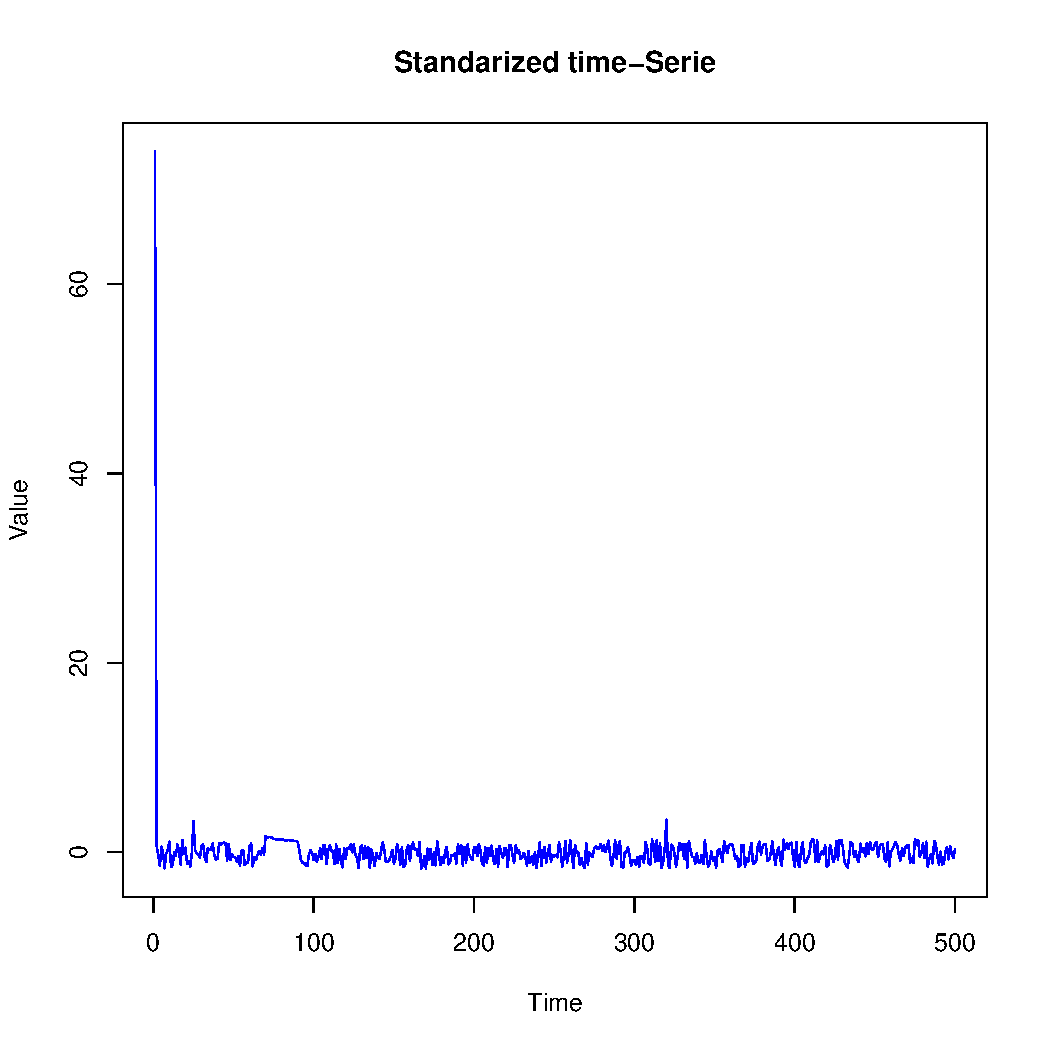
\includegraphics[width=\maxwidth]{figure/Predict-1} 
\end{knitrout}

As a prediction model EORELM-AD is used and it is initialized as in Example 3.

\begin{knitrout}
\definecolor{shadecolor}{rgb}{0.969, 0.969, 0.969}\color{fgcolor}\begin{kframe}
\begin{alltt}
\hlstd{detector} \hlkwb{<-} \hlstd{EorelmAD}\hlopt{$}\hlkwd{new}\hlstd{(}
  \hlkwc{n.train} \hlstd{=} \hlnum{20}\hlstd{,}
  \hlkwc{numLags} \hlstd{=} \hlnum{10}\hlstd{,}
  \hlkwc{numHiddenNeurons} \hlstd{=} \hlkwd{c}\hlstd{(}\hlnum{20}\hlstd{),}
  \hlkwc{normMethod} \hlstd{=} \hlkwa{NULL}\hlstd{,}
  \hlkwc{outlierMethod} \hlstd{=} \hlstr{"DSS"}\hlstd{,}
  \hlkwc{threshold} \hlstd{=} \hlnum{0.5}
\hlstd{)}
\end{alltt}
\end{kframe}
\end{knitrout}

Then the prediction on the the whole dataset is carried out.

\begin{knitrout}
\definecolor{shadecolor}{rgb}{0.969, 0.969, 0.969}\color{fgcolor}\begin{kframe}
\begin{alltt}
\hlstd{result} \hlkwb{<-} \hlstd{detector}\hlopt{$}\hlkwd{predict}\hlstd{(online_norm_value)}
\hlstd{res} \hlkwb{<-} \hlkwd{cbind}\hlstd{(df, result)}
\end{alltt}
\end{kframe}
\end{knitrout}

To show how to use the online scoring function in the following, we calculate the anomaly score from the prediction error obtained in the previous run.

\begin{knitrout}
\definecolor{shadecolor}{rgb}{0.969, 0.969, 0.969}\color{fgcolor}\begin{kframe}
\begin{alltt}
  \hlstd{scorer} \hlkwb{<-} \hlstd{DynamicSigmaScorer}\hlopt{$}\hlkwd{new}\hlstd{()}
  \hlstd{anomaly.score} \hlkwb{<-} \hlkwd{sapply}\hlstd{(res}\hlopt{$}\hlstd{error, scorer}\hlopt{$}\hlstd{computeScore)}
\end{alltt}
\end{kframe}
\end{knitrout}

Finally, it can be seen that the score obtained by DynamicSigmaScoring and the score obtained by EORELM-AD are exactly the same.

\begin{knitrout}
\definecolor{shadecolor}{rgb}{0.969, 0.969, 0.969}\color{fgcolor}\begin{kframe}
\begin{alltt}
 \hlkwd{setdiff}\hlstd{(anomaly.score, res}\hlopt{$}\hlstd{anomaly.score)}
\end{alltt}
\begin{verbatim}
## numeric(0)
\end{verbatim}
\begin{alltt}
 \hlkwd{cbind}\hlstd{(}\hlstr{"score"} \hlstd{= anomaly.score,} \hlstr{"res-score"} \hlstd{= res}\hlopt{$}\hlstd{anomaly.score)[}\hlnum{100}\hlopt{:}\hlnum{105}\hlstd{,]}
\end{alltt}
\begin{verbatim}
##             score    res-score
## [1,] 0.0044822023 0.0044822023
## [2,] 0.0110590130 0.0110590130
## [3,] 0.0240821506 0.0240821506
## [4,] 0.0135302591 0.0135302591
## [5,] 0.0037784959 0.0037784959
## [6,] 0.0007961603 0.0007961603
\end{verbatim}
\end{kframe}
\end{knitrout}


\subsection{Most useful functions}
\label{sec:summaryfunctions}

\begin{table}[htbp]
  \centering
  \resizebox{\textwidth}{!}{%
  \begin{tabular}{llll}
    \hline
    \textbf{Functionality} & \textbf{Description} & \textbf{Offline} & \textbf{Online} \\ \hline
    \multirow{6}{*}{Detectors} & PEWMA & CpPewma & IpPewma \\
     & SD-EWMA & CpSdEwma & IpSdEwma \\
     & TSSD-EWMA & CpTsSdEwma & IpTsSdEwma \\
     & KNN-ICAD & CpKnnCad(ncm.type = "ICAD") & IpKnnCad(ncm.type = "ICAD") \\
     & KNN-LDCD & CpKnnCad(ncm.type = "LDCD") & IpKnnCad(ncm.type = "LDCD") \\
     & CAD-OSE & ContextualAnomalyDetector & ContextualAnomalyDetector \\
     & EORELM-AD (R6) & EorelmAD & EorelmAD \\ \hline
    \multirow{2}{*}{NAB score} & Get score & GetDetectorScore & \multicolumn{1}{c}{-} \\
     & Normalize score: & \begin{tabular}[c]{@{}l@{}}NormalizeScore\\
     GetNullAndPerfectScores\end{tabular} & \multicolumn{1}{c}{-} \\ \hline
    \begin{tabular}[c]{@{}l@{}}False Positve \\
    Reduction\end{tabular} & False positive reduction & ReduceAnomalies & ReduceAnomalies \\ \hline
    Visualization & \begin{tabular}[c]{@{}l@{}}Static or \\
    interactive visualizations\end{tabular} & PlotDetections & \multicolumn{1}{c}{-} \\ \hline
    \multirow{4}{*}{Online normalization}
     & Dynamic normalization (R6) & DynamicNormalizer & DynamicNormalizer \\
     & Window normalization (R6) & WindowNormalizer & WindowNormalizer \\
     & One-pass adaptive normalization (R6) & AdaptiveNormalizer & AdaptiveNormalizer \\
     & One-pass adaptive min-max normalization (R6) & AdaptiveNormalizer2 & AdaptiveNormalizer2 \\ \hline
     \multirow{4}{*}{Online scoring}
     & Anomaly likelihood (R6) & AnomalyLikelihoodScorer & AnomalyLikelihoodScorer \\
     & Dynamic threshold (R6) & DynamicThresholdScorer & DynamicThresholdScorer \\
     & Sigma scoring (R6) & SigmaScorer & SigmaScorer \\
     & Dynamic sigma scoring (R6) & DynamicSigmaScorer & DynamicSigmaScorer \\ \hline
  \end{tabular}%
  }
\end{table}

\section{Summary}\label{sec:summary}

In this paper, we present the \pkg{otsad} package for R. This package fully meets the demand for anomaly detection algorithms over univariate time series in online environments. With this package we tackle with the ability to work with stationary and non-stationary data. We also provide algorithms of the two detection techniques (evolving and window based) that are gaining strength on research.

As a future job, we propose to maintain and add functionalities to our \pkg{otsad} package, i.e. provide more sophisticated false positive reduction techniques and incorporate them into algorithms.

\bibliography{otsad}
\bibliographystyle{plain}

\end{document}
